\chapter{Introduction to Neutrino Physics}
\label{c:theoryIntro}

\section{Research Goals}
The research in this thesis describes the construction of a prototype Magnetized Iron Neutrino Detector (Baby MIND) at the European Organization for Nuclear Research (CERN), its performance to reconstruct charged particle interactions and determine their charge, carried out at a test beam at CERN, and the measurement of neutrino interactions with the WAGASCI detector, carried out at the neutrino beam line at the Japan Proton Accelerator Research Complex (J-PARC). Before describing the research carried out in detail, this first chapter contains a short introduction to neutrino physics.
%and determine the performance of the detector to reconstruct charged particle tracks at a test beam at CERN and neutrino interactions with our collaborators in the WAGASCI collaboration at a neutrino beam line at the Japan Proton Accelerator Research Complex (J-PARC). %This is discussed further in chapter~\ref{c:WAGASCI}.

%This research aims to construct a prototype Magnetized Iron Neutrino Detector (Baby MIND) at the European Organization for Nuclear Research (CERN) and understand the performance of the detector to reconstruct charged particle tracks at a test beam at CERN and neutrino interactions with our collaborators in the WAGASCI collaboration at a neutrino beam at the JPARC facility in Japan. This is discussed further in chapter~\ref{c:WAGASCI}.

\section{Neutrino discovery}\label{section:Theory}
While measuring radioactive beta decay, in the first two decades of the 20th century, from bombarding beryllium with alpha particles from polonium, physicists discovered what was then an anomaly. At the time it was thought that beta decay occurred as a two body process in which a neutron ($n$) decays to a proton ($p$) and electron ($e^-$). If this were the case, the energy of the proton and electron should be discrete and add up to the energy of the neutron. However experiments showed that the electron had a continuous spectrum of energy values, violating the energy conservation law, as seen in \FigRef{fig:betaeng}~\cite{89Neary71}. In order to solve this anomaly, a third particle, the neutrino ($\nu$), was postulated by Wolfgang Pauli \cite{4Pauli:Online} and then incorporated into the beta decay by Enrico Fermi \cite{5Wilson}. The neutrino was postulated as a neutral particle with mass of less than 1\% of the proton mass and a spin of 1/2. For consistency, the particle produced in the beta decay is relabelled as the electron antineutrino, $\bar{\nu_e}$, in order to conserve lepton number. The addition of another particle changed the decay to $n \rightarrow p + e^- + \bar{\nu_e}$ and introduced the weak interaction model, as seen in \FigRef{fig:beta}. 

\begin{figure}[h!]
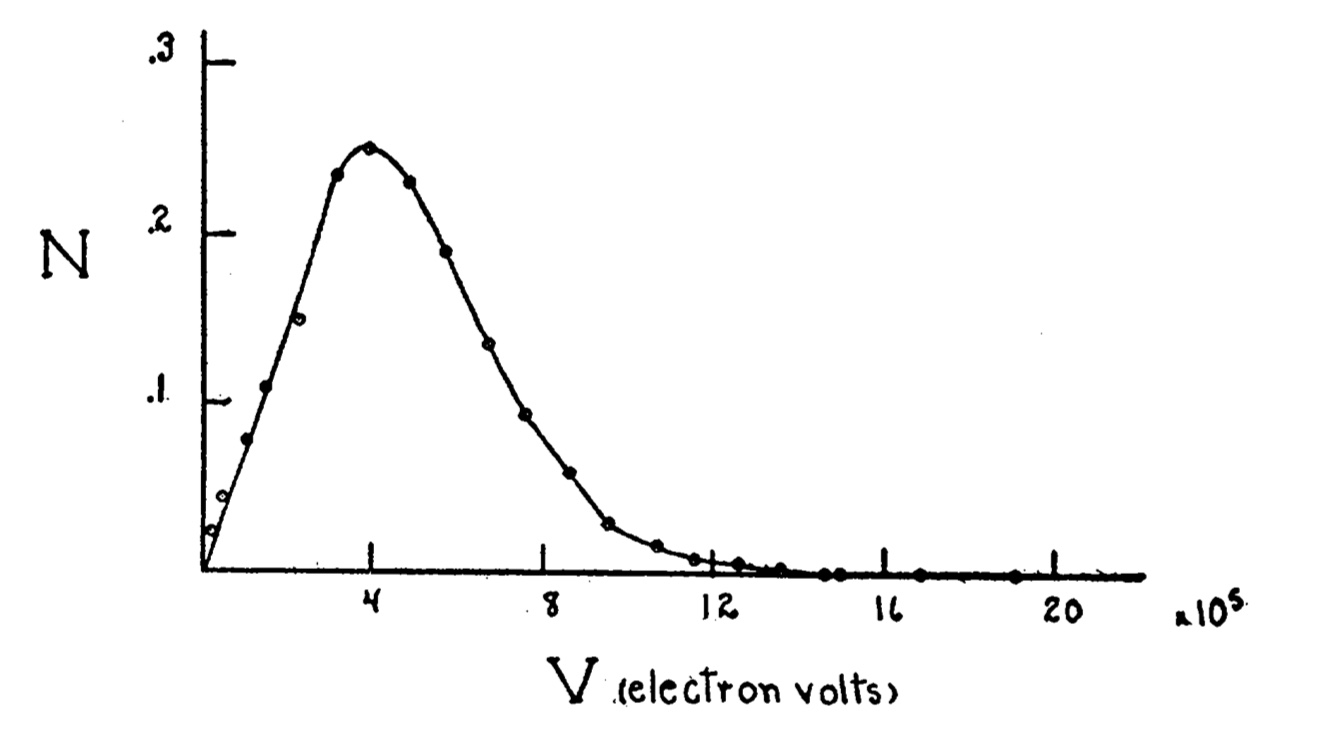
\includegraphics[width=\textwidth]{figures/betaRadium.jpeg}
\caption{The kinetic energy spectrum of the emitted electron from beta decay from a Radium-E source~\cite{RadiumE}. If no anti-neutrino were emitted a single electron volt(s) value would be expected.}
\label{fig:betaeng}
\end{figure}

\begin{figure}[h!]
\centering
\begin{subfigure}{.5\textwidth}
  \centering
  \begin{fmffile}{badBeta}
\begin{fmfgraph*}(120,80)
\fmfstraight
\fmfleft{i1,i2,o1}
\fmfright{o2}

\fmf{fermion}{i1,v1}
\fmf{fermion}{v1,o1}

%fmf{boson}{v1,v2}
\fmf{fermion}{v1,o2}

\fmflabel{n}{i1}
\fmflabel{p}{o1}
\fmflabel{$e^{-}$}{o2}
\end{fmfgraph*}
\end{fmffile}
\vspace{2mm}
  \caption{The initially assumed beta decay}
  %\label{fig:sub1}
\end{subfigure}%
\begin{subfigure}{.5\textwidth}
  \centering
  \begin{fmffile}{beta}
\begin{fmfgraph*}(120,80)
\fmfstraight
\fmfleft{i1,i2,o1}
\fmfright{o2,o3}

\fmf{fermion}{i1,v1}
\fmf{fermion}{v1,o1}

\fmf{boson}{v1,v2}
\fmf{fermion}{v2,o2}
\fmf{fermion}{o3,v2}

\fmflabel{n}{i1}
\fmflabel{p}{o1}
\fmflabel{$e^{-}$}{o2}
\fmflabel{$\bar{\nu}_e$}{o3}
\end{fmfgraph*}
\end{fmffile}
\vspace{2mm}
  \caption{Correct beta decay}
  %\label{fig:sub2}
\end{subfigure}
\vspace{2mm}
\caption{Feynman diagrams showing beta decay.}
\label{fig:beta}
\end{figure}

It would take another twenty years until the neutrino was experimentally discovered by the Savannah river reactor experiment in 1956~\cite{6Reines} where neutrinos from a nuclear reactor were detected in 300 litres of liquid scintillator and cadmium. Fredrick Reines was awarded the Nobel prize in 1995 for his leading role in this experiment.

After the discovery of the electron neutrino ($\nu_e$), several neutrino experiments were performed and led to the discovery of two other neutrino types/flavours, the muon neutrino ($\nu_\mu$) and the tau neutrino ($\nu_\tau$)~\cite{7Danby, 8Perl, Fix1}.


\section{Standard Model}\label{section:SM}

\subsection{Quantum Electrodynamics}

\if{0}
\textbf{Put in V-A theory here? weak interaction model. Fermi theory?}
\textbf{Expand with parity violation etc etc?}

Explain QED, use this plus experiments (chirality etc) to introduce a modified QED for weak interactions, V-A theory. Using this find neutral current experiment which is not in V-A theory leading to electroweak unification.
Start with dirac lagrangian, impose local gauge invariance produces a massless vector field A, set A as the photon field and we are done! 
Very few details, more in Peskin and Schroeder and other books.
\textbf{Mix in experiments!}
\fi

To describe neutrino interactions it is worth building a theory to try to describe the processes involved. Starting with the generalized and relativistic version of the Schr\"{o}dinger equation, the Dirac equation:
\begin{equation}
\sum_\mu (i\gamma^\mu \partial_\mu - m)\psi(x) = 0
\end{equation}
where $\gamma$ are the so called Dirac matrices and the sum over $\mu$ is often removed using the Einstein notation requiring summation over repeated indices.

As with all quantum mechanical equations this allows us to define $\psi(x)$ as a quantum field or state.

After taking Lorentz-invariance into account the Dirac Lagrangian can be written as:
\begin{equation}
\mathcal{L} = \bar{\psi}(i\gamma^\mu\partial_\mu-m)\psi
\end{equation}
where the Euler-Lagrange equation for $\bar{\psi}$ reproduces the Dirac equation.

The Lagrangian is so far correct, however from a physical point of view the equation also needs to be invariant under a phase shift, the so called gauge transformation $\psi \rightarrow e^{i\theta(x)}\psi$. This requires the addition of an extra term to remove the terms that prevent gauge invariance, providing the full Dirac Lagrangian as:

\begin{equation}
\mathcal{L} = \bar{\psi}(i\gamma^\mu\partial_\mu-m)\psi -q\bar{\psi}\gamma^\mu\psi\epsilon_\mu \equiv \mathcal{L}_{Dirac}
\end{equation}
with $\epsilon_\mu$ being a new field which must be gauge invariant and $q$ a conserved quantity, a numerical constant.

There is now a mathematical framework to describe quantum states or particles in a vacuum, and for a particle interacting with an electromagnetic field by combining $\mathcal{L}_{Dirac}$ with the classical $\mathcal{L}_{Maxwell} = \frac{-1}{4}F_{\mu\nu}F^{\mu\nu} $ with $F^{\mu\nu} = \partial^\mu A^\nu - \partial^\nu A^\mu$ where $A_\mu$ is the electromagnetic vector potential, a four-vector combination of the electric potential and magnetic potential. 

This produces the following Lagrangian:
\begin{equation}
\mathcal{L} = \mathcal{L}_{Dirac} + \mathcal{L}_{Maxwell} = \bar{\psi}(i\gamma^\mu\partial_\mu-m)\psi -q\bar{\psi}\gamma^\mu\psi\epsilon_\mu - \frac{1}{4}F_{\mu\nu}F^{\mu\nu}
\end{equation}

There is nothing preventing us from choosing our previous field $\epsilon$ as the electromagnetic vector potential $A$ and choosing $q$ as the electron charge $e$ to produce the experimentally verified Lagrangian for quantum and electromagnetic interactions or Quantum ElectroDynamics (QED):

\begin{equation}
\mathcal{L}_{QED} \equiv \bar{\psi}(i\gamma^\mu\partial_\mu-m)\psi -e\bar{\psi}\gamma^\mu\psi A\mu - \frac{1}{4}F_{\mu\nu}F^{\mu\nu}
\end{equation}
This can be simplified by introducing the gauge covariant derivative $D_\mu \equiv \partial_\mu + ieA_\mu$ and the slash notation as $\displaystyle{\not} D = \gamma^\mu D_\mu$. This produces the simplified QED Lagrangian as:
\begin{equation}
\mathcal{L}_{QED} = \bar{\psi}(i\gamma^\mu \displaystyle{\not} D_\mu-m)\psi - \frac{1}{4}F_{\mu\nu}F^{\mu\nu}
\end{equation}

%\textbf{Add example of interaction?} 
%\textbf{electron muon scattering? and introducing Feynman diagrams}

\subsection{Weak interactions}

Based on the experiments relating to $\beta$-decay, Fermi hypothesised that the Lagrangian for weak interactions should be similar to the QED Lagrangian. To handle the observed differences, a constant is added $G_F$ to replace the electron charge, and mass term is removed.The assumption was made that the neutrinos were massless. QED contains the covariant multiplier $\gamma^\mu$ meaning that it transforms as a vector, which was confirmed by experiments. The transformation structure  of weak interactions was not known and, a priori, anything could be mathematically possibly. However, the absence of Fierz interference terms, parity violation and the Goldhaber helicity experiment~\cite{1Helicity} made it clear that the interactions had to transform as vectors and axial vectors giving the term $\gamma^\mu - \gamma^\mu \gamma^5 =  \gamma^\mu (1- \gamma^5)$ and also providing the theory with its name: V-A theory~\cite{90Feynman}. 

This produced a Lagrangian in the form of 
\begin{equation}
\mathcal{L} = \frac{G_F}{\sqrt{2}}J_L \cdot J_H
\end{equation}
with $J_L$ as the current describing interactions with leptons and $J_H$ describing interactions with hadrons (up and down quarks instead of protons and neutrinos). The Fermi constant $G_F$ was also added to substitute the electron charge. The currents were initially of the form:
\begin{equation}
J_L = \bar{\psi}_e(x)\gamma^\mu (1-\gamma_5) \psi_\nu(x)
\end{equation}
containing only the electron, and then expanded by adding more terms containing future particles. For the hadrons it could either be written for quarks as:
\begin{equation}
J_H = \bar{\psi}_u(x)\gamma^\mu (1-\gamma_5) \psi_d(x)
\end{equation}
or for protons and neutrons as:
\begin{equation}
J_H = \bar{\psi}_p(x)\gamma^\mu (g_V-g_A\gamma_5) \psi_n(x)
\end{equation}
where $g_V$ and $g_A$ are constants relating to strong interactions and have to be determined experimentally along with $G_F$.

%\pagebreak
\subsection{Glasgow-Weinberg-Salam Theory}\label{subsection:SMN}
V-A theory works well in practice but does not create a Gauge theory connecting to an underlying field, such as QED does. It is also based on the interacting particles not having mass which does not explain the observed masses of the weak interaction particles, W bosons. There is also no explanation for any neutral interactions which were observed~\cite{91Hasert} and introduced a massive Z boson. Group theory describes that any unitary group $U(N)$ has $N^2 -1$ generators. The special unitary groups $SU(N)$ were investigated to include interactions mediated by other bosons, in analogy with the $SU(1)$ group that successfully describes QED.

%This is also the case for groups with the determinant 1 denoted special S. Based on the SU(1) group from QED, the easiest group to handle the other bosons becomes SU(2). 

Glashow-Weinberg-Salam (GWS) took the success of the V-A theory and modified it to make a Gauge theory out of it, Quantum Flavour Dynamics (QFD) with massive intermediate vector bosons W and Z, basing it on the SU(2) group~\cite{92Weinberg, 93Salam, 94Glashow}. It was also easy to see that QFD and QED could be unified as an SU(2) group can be made invariant under U(1) by adding an extra term. By choosing this constant term correctly QFD and QED were unified into the Electro-weak theory.

The experiment by \citeauthor{1Helicity} concluded that neutrinos only exist in a left-handed chiral state, meaning that momentum and spin are oppositely aligned~\cite{1Helicity}. They also concluded that anti-neutrinos only exist in the right handed state. In the initial or unexpanded SM, \cite{34doi:10.1142/9789812562203_0002}, only fermions which have both chiral states have mass through the Brout\hyp{}Englert\hyp{}Higgs mechanism~\cite{35Higgs}. At the time this led to the definition of the neutrino as a massless particle, however in \SubSectionRef{subsection:Neutrinomassandoscillation} it will be shown that neutrino oscillations require at least one of the neutrinos to have mass. This indicates that the SM needs to be extended to account for this new physics.

%\textbf{Glashow-Weinberg-Salam (GWS) took the success of the V-A theory and modified it to make a Gauge theory out of it. Massive Ws and Z. Add left/right doublets and singlets? Required for no experimental right-handed neutrinos. Higgs is a SU(2) Left doublet. Properly write in that we are creating an SU(2) because U(2) makes no sense? but U(1) Aha! U(1) in QED could be SU(1), but U(1) is more general and explains it well. For QFD, require SU since basing it on Pauli matrices.}

The work by GWS will now be briefly detailed. Since experiments require 3 bosons and interaction modes, one can start with a simple field and make it SU(2). Initially the Lagrangian can naively be taken as that of a complex scalar field coupled to the electromagnetic field (and itself) as:
\begin{equation}
\mathcal{L} = - \frac{1}{4} F_{\mu\nu}F^{\mu\nu} + |D_\mu \phi |^2  -V(\phi)
\end{equation}
where $D_\mu$ is the covariant derivative from QED, $D_\mu = \partial_\mu +ieA_\mu$ and a potential V will be discussed shortly as a way of adding mass to the theory.

Following the procedure performed to produce QED and requiring gauge invariance implies that the covariant derivative needs to be changed, requiring a field for each of the so called generators or each of the bosons. This requires 3 new fields aside from the QED/photon field. This changes the covariant derivative in the following way,
\begin{equation}
D_\mu = \partial_\mu - ig S^a_\mu \frac{\sigma^a}{2} - \frac{1}{2}g' A_\mu
\end{equation}
where $g'$ is now the new coupling to the photon field and $g$ is the coupling to our new fields $S$, while $\sigma_a$ are the Pauli matrices with $a$ the index that can take the values 1, 2 and 3.

At this stage there are enough fields to produce the bosons required, however there needs to be a way of making all but the photon field massive.

V is chosen in a way such that it produces a massive Goldstone boson~\cite{80Goldstone} and so that it is also gauge invariant. This gives V as:
\begin{equation}
V(\phi) = - \mu^2 \phi^{*}\phi + \frac{\lambda}{2}(\phi^{*}\phi)^2
\end{equation}
where $\mu$ is a parameter.
If $\mu^2 <0$ it will produce a massive boson, this is also a way of producing a massive photon in QED, however if $\mu^2 >0$ then a spontaneously symmetry breaking is produced and $\phi$ can be split into a real and complex part where the real part will have mass but the complex will not. Essentially this breaks down the $SU(2) \times U(1)$ to a $U(1)$ theory. Therefore it produces one massless vector boson (the photon field $A$), three massive vectors boson fields (the $S$ fields) and a vacuum expectation value $v$ relating to the physical Higgs scalar.

The potential can be chosen, within the symmetry breaking as the Higgs potential~\cite{35Higgs}:
\begin{equation}
\langle \phi \rangle = \frac{1}{\sqrt{2}}
\begin{pmatrix}
    0\\
    v
\end{pmatrix}
\end{equation}

The mass related to each of these fields arrives from the $|D_\mu \phi |^2$ term in the Lagrangian. This can be explicitly seen, using the Higgs potential and $\phi^* |D_\mu \phi |^2 \phi$. Using the fact that the potential is a constant and cancelling signs produces:
\begin{equation}
V(\phi) = \begin{pmatrix}
    0 & v
\end{pmatrix}
(
g S^a_\mu \frac{\sigma^a}{2} + \frac{1}{2}g' A_\mu
)
(
g S^{b\mu} \frac{\sigma^b}{2} + \frac{1}{2}g' A^\mu
)
\begin{pmatrix}
    0\\
    v
\end{pmatrix}
\end{equation}
Using the properties of Pauli matrices this can be rewritten as:
\begin{equation}
V(\phi) = \frac{1}{2}\frac{v^2}{4}\lbrace g^2 (S_\mu^1)^2 + g^2 (S_\mu^2)^2 + (-gS^3_\mu+g' A_\mu)^2 \rbrace
\end{equation}
These results can be modified to show how mass is added to fermions as well.

The terms corresponding to the factors $g$ and $g’$ can be combined to produce four different field combinations that result in bosons with different masses, three are massive bosons and one is massless:
\begin{align}
W^\pm &= \frac{1}{\sqrt{2}}(S_\mu^1 \mp S_\mu^2)\\
Z_\mu &= \frac{1}{\sqrt{g^2+g'^2}}(gS_\mu^3 - g' A_\mu)\\
\gamma_\mu &= \frac{1}{\sqrt{g^2+g'^2}}(g'S_\mu^3 + g A_\mu).
\end{align}
The masses for the bosons are  $m_W = g\frac{v}{2}$, $m_Z = \sqrt{g^2+g'^2}\frac{v}{2}$ and $m_\gamma = 0$. By defining a weak mixing angle, the Wienberg angle, a relationship between these fields can be defined as:
\begin{equation}
\begin{pmatrix}
    Z\\
 \gamma
\end{pmatrix}
=
\begin{pmatrix}
    \cos(\theta_W) & -\sin(\theta_W)\\
    \sin(\theta_W) & \cos(\theta_W)\\
\end{pmatrix}
\begin{pmatrix}
    S^3\\
  A
\end{pmatrix}
\end{equation}
where $\cos(\theta_W) = \frac{g}{\sqrt{g^2+g'^2}}$ and $\sin(\theta_W) = \frac{g'}{\sqrt{g^2+g'^2}}$. This also provides a relationship between the W and Z masses, as $m_W = m_Z \cos(\theta_W)$. To also ensure that QED is properly included in this theory the terms in front of the $\gamma$-field must be equal to the electron charge providing the following relationship:
$e = g \sin(\theta_W) = g' \cos(\theta_W)$

This allows the final interaction Lagrangian to be written as:
\begin{align}
\mathcal{L}_{int}&=i\frac{g}{\sqrt{2}}[j_\mu^{(+)}W^{\mu-}+j_\mu^{(-)}W^{\mu+}]\\ \nonumber
&+i[g\cos\theta_Wj_\mu^{(3)}-g'\sin\theta_Wj_\mu^{(Y/2)}]Z^\mu\\ \nonumber
&+i[g\sin\theta_Wj_\mu^{(3)}+g'\cos\theta_Wj_\mu^{(Y/2)}]\gamma^\mu
\end{align}
or simplified as 
\begin{align}
\mathcal{L}_{int}&=i\frac{g}{\sqrt{2}}[j_\mu^{(+)}W^{\mu-}+j_\mu^{(-)}W^{\mu+}]\\ \nonumber
&+i[g\cos\theta_Wj_\mu^{(3)}-g'\sin\theta_Wj_\mu^{(Y/2)}]Z^\mu\\ \nonumber
&+ie[j_\mu^{(3)}+j_\mu^{(Y/2)}]\gamma^\mu
\end{align}
where $j_{\mu}^{(a)}$ are the different currents for each of the interactions. As an example, for the interaction between an electron and a neutrino, a purely week interaction, the currents are written as:
\begin{align}
j_\mu^{(W+)}&=\frac{1}{2}\bar{\nu}_e\gamma_\mu(1-\gamma_5)e\\
j_\mu^{(W-)}&=\frac{1}{2}\bar{e}\gamma_\mu(1-\gamma_5)\nu_e\\
j_\mu^{(Z)}&=\frac{1}{2}\bar{\nu}_e\gamma_\mu(1-\gamma_5)\nu_e-\frac{1}{2}\bar{e}\gamma_\mu(1-\gamma_5)e+2\sin^2\theta_W\bar{e}\gamma_\mu e\\
j_\mu^{(3)}&=0\\
j_\mu^{(Y/2)}&=0.
\end{align}
Comparing the formula for $j_\mu^{(Z)}$ from the electroweak theory above, and from V-A theory, $j_\mu^{(Z)}=\frac{1}{2}\bar{\nu}_e\gamma_\mu(1-\gamma_5)\nu_e+\bar{e}\gamma_\mu(g_V-g_A\gamma_5)e$, provides a relation between the $g_V$ and $g_A$ and the Weinberg angles as $g_V=-\frac{1}{2}+2\sin^2\theta_W$ and $g_A = -\frac{1}{2}$. Given that both the currents for both W and Z are non-zero means that electrons and neutrinos should have interactions through all three bosons. Looking in detail it can be seen that both of the W currents couple anti-neutrino to electron or vice-versa but the Z current only couples the particles to themselves. This means that the W currents carry charge and thus are named charge-current interactions compared to the Z current where this is not the case and have been named neutral-current interactions.

%The final resulting theory has added massive bosons, explains and provides a framework for electro-weak interactions and mass.

%Interactions, probabilities. CC, other interaction types, NC, QE. Define and explain cross-sections and probabilities. What does the theory predict?

Finally to produce the full Standard Model requires the strong interaction QCD which will not be described in this thesis, and details can be found in~\cite{13PDG} among others. 

The Standard Model of particle physics (SM) categorizes all the fundamental particles that have been discovered experimentally and the mathematics of their properties and how they interact \cite{32Burchan:1995, 38griffiths}. 

The particles in SM, seen in \FigRef{fig:standardModel}, can be split into two different types, fermions and gauge bosons, characterised by their half-integer and integer spin. Fermions can be further split depending on whether they experience strong interactions or not, with quarks undergoing strong interactions and having fractional charge, and leptons that do not see the strong force and have integer charge. Gauge bosons are the force mediators for the particle interactions while the Higgs boson is the only scalar, spin 0, particle in the SM, responsible for symmetry breaking and giving mass to all particles~\cite{35Higgs}.





\begin{figure}[h!]
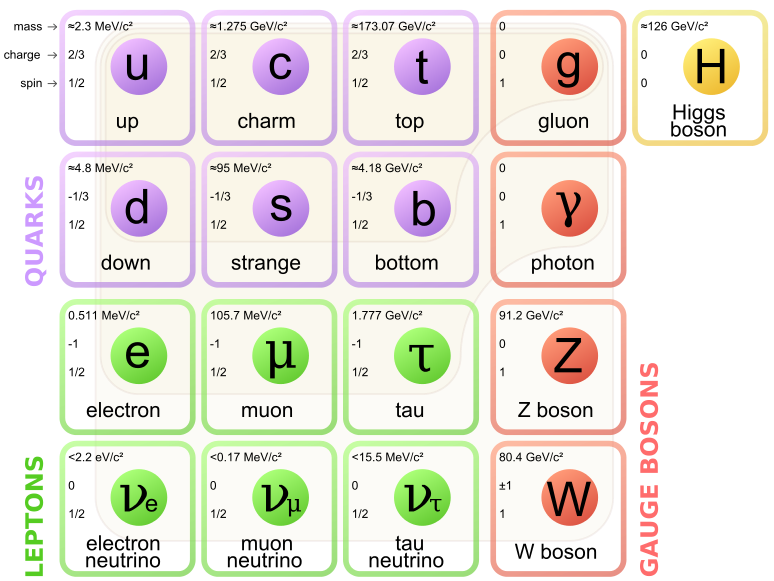
\includegraphics[width=0.7\textwidth]{figures/Standard_Model_of_Elementary_Particles.png}
\caption{The standard model of particle physics where the three first columns represent the so called generations, starting with the first. \cite{33wiki1:Online}}
\label{fig:standardModel}
\end{figure}

\if{0}
Made it su2  because? SM is based on it but why? Number of particles?

Why only left doublets and right singlets? Did they know? Massless particles? From isospin in strong?

The elementary particles are arranged as doublets for chiral left-handed fields and singlets for right-handed fields in the form.

\begin{equation}
\begin{pmatrix}
    u\\
    d'
\end{pmatrix}_L
\begin{pmatrix}
    c\\
    s'
\end{pmatrix}_L
\begin{pmatrix}
    t\\
    b'
\end{pmatrix}_L
\begin{pmatrix}
    e\\
    \nu_e
\end{pmatrix}_L
\begin{pmatrix}
    \mu\\
    \nu_\mu
\end{pmatrix}_L
\begin{pmatrix}
    \tau\\
    \nu_\tau
\end{pmatrix}_L
\end{equation}
and $u_R$,  $d_R$, $s_R$, $c_R$, $b_R$, $t_R$, $e_R$, $\mu_R$, $\tau_R$. 
Note how the neutrino is not modelled with a right handed component as the existence of right handed neutrinos was ruled out by \textbf{EXPERIMENT} before this theory was designed.

More details
\fi

\pagebreak

\section{Neutrino interactions}\label{subsection:Neutrino interactions}
%The described theory can be used to describe how neutrinos interact and with what.

Neutrino interactions are split into two different types depending on which boson mediates the interaction.
Charge Current (CC) interactions change the final state quarks or leptons by one unit of electric charge and are mediated by the $W^+$ and $W^-$ bosons while Neutral Current (NC) interactions do not change the charge and are mediated by a $Z^0$ boson. 
To look at possible interactions of neutrinos described in the Standard Model of particle physics, one needs to look at the quantum field theory description of the interactions, as was described in section~\ref{section:SM} and details can be found in, among others~\cite{3Peskin, 2Hallsjo}.  %The further subsections have been split depending on what interaction particle is involved.

\subsection{Neutrino-electron interactions}

%\textbf{New material}

%Through the theory it is clear that neutrinos should interact with electrons. Electrons are a fundamental particle meaning that the interaction can be seen as pointlike interactions.

Neutrinos interact with electrons by Charge Current and Neutral Current interactions. Since electrons are fundamental particles, their interactions are point-like.

When it comes to neutrino and electron interactions, experimentally only the following have been observed:

Lagrangian for NC scattering, $\nu_x e \rightarrow \nu_x e$:
\begin{equation}
\mathcal{L}=-\frac{G_F}{\sqrt{2}} \left[ \bar{\nu_x}\gamma_\alpha (1-\gamma_5)\nu_x \right] \left[ \bar{e} \gamma_\alpha (g_V-g_A \gamma_5)e \right]
\end{equation}

with the constants as defined previously. The Fermi constant $G_F$, the Weinberg angle $\theta_W$ and where $g_V$ and $g_A$ are constants relating to strong interactions from V-A theory.

Lagrangian for CC scattering, $\nu_x e \rightarrow \nu_e x$:
\begin{equation}
\mathcal{L}=-\frac{G_F}{\sqrt{2}} \left[ \bar{\nu_x}\gamma_\alpha (1-\gamma_5)x\right] \left[ \bar{\nu_e}\gamma_\alpha (1-\gamma_5)e \right]
\end{equation}

The cross sections are calculated by first calculating the  interaction amplitude by using the initial and final states to evaluate the Lagrangian. This amplitude can then be related to a derivative of the cross-section which can be integrated to provide the final cross section. The details can be found in~\cite{3Peskin}.

The various processes involving an electron as an initial state with their calculated cross sections can be seen in table~\ref{tab:electronproc} where the variable $s$ is the Mandelstam variable, $s=(p_{\nu_\mu} + p_e)^2 = 2m_e E_{\nu_\mu}$

\begin{table}[h!]
\centering
\caption{Neutrino interactions with electrons.}
\label{tab:electronproc}
\begin{tabular}{|l|l|l|}
 \hline
Type & Process & Cross-section \\
 \hline
CC interaction & $\nu_\mu + e^- \rightarrow \mu^- + \nu_e$  & $\frac{G_F^2 s}{\pi}$\\
CC+NC Scattering & $\nu_e + e^- \rightarrow \nu_e + e^-$ & $\frac{G_F^2 s}{4\pi} \left[ (2\sin^2 \theta_W -1){}^2 +\frac{4}{3}\sin^2 \theta_W \right]$\\ 
CC+NC Scattering & $\bar{\nu_e} + e^- \rightarrow \bar{\nu_e} + e^-$ & $\frac{G_F^2 s}{4\pi} \left[ \frac{1}{3}(2\sin^2 \theta_W +1){}^2 +4\sin^2 \theta_W \right]$ \\
NC Scattering & $\nu_\mu + e^- \rightarrow \nu_\mu + e^-$ & $\frac{G_F^2 s}{4\pi} \left[ (2\sin^2 \theta_W -1){}^2 +\frac{4}{3}\sin^2 \theta_W \right]$ \\
NC Scattering & $\bar{\nu_\mu} + e^- \rightarrow \bar{\nu_\mu} + e^-$ &$\frac{G_F^2 s}{4\pi} \left[ \frac{1}{3}(2\sin^2 \theta_W -1){}^2 +4\sin^2 \theta_W \right]$ \\
Neutrino pair production & $e^+ + e^- \rightarrow \nu_e + \bar{\nu_e}$ & $\frac{G_F^2 s}{12\pi} \left[ \frac{1}{2} + 2\sin^2 \theta_W + 4\sin^4 \theta_W \right]$ \\
Neutrino pair production & $e^+ + e^- \rightarrow \nu_\mu + \bar{\nu_\mu}$ & $\frac{G_F^2 s}{12\pi} \left[ \frac{1}{2} - 2\sin^2 \theta_W + 4\sin^4 \theta_W \right]$ \\
 \hline
\end{tabular}
\end{table}

To make it simpler for calculations and visualization these interactions have been plotted as Feynman diagrams in~\FigRef{fig:einteractions1}, \FigRef{fig:einteractions2} and \FigRef{fig:einteractions3}.

\begin{figure}[h!]
\vspace{2mm}
\centering
\begin{subfigure}{.5\textwidth}
  \centering
  \begin{fmffile}{TEST}
\begin{fmfgraph*}(120,80)
\fmfstraight
\fmfleft{i1,i2}
\fmfright{o1,o2}

\fmf{fermion}{i1,v1,o1}
%\fmf{fermion}{v1,o1}
\fmf{fermion}{i2,v2,o2}
\fmf{boson,label=$W^-$}{v1,v2}
%\fmf{fermion}{o2,v2}
%\fmf{fermion}{v2,o3}
\fmflabel{$e^{-}$}{i1}
\fmflabel{$\nu_{\mu}/\nu_{e}$}{i2}
\fmflabel{$\nu_{e}$}{o1}
\fmflabel{$\mu^-/e^-$}{o2}
\end{fmfgraph*}
\end{fmffile}
\end{subfigure}%
\begin{subfigure}{.5\textwidth}
  \centering
  \begin{fmffile}{TEST2}
\begin{fmfgraph*}(120,80)
\fmfstraight
\fmfleft{i1,o1}
\fmfright{i2,o2}

\fmf{fermion}{v1,o1}
\fmf{fermion}{i1,v1}

\fmf{boson,label=$W^+$}{v1,v2}
\fmf{fermion}{i2,v2}
\fmf{fermion}{v2,o2}

\fmflabel{$e^{-}$}{i1}
\fmflabel{$\bar{\nu_e}$}{o1}
\fmflabel{$\bar{\nu_e}$}{i2}
\fmflabel{$e^{-}$}{o2}
\end{fmfgraph*}
\end{fmffile}
\end{subfigure}
\vspace{2mm}
\caption{Charge current interaction between neutrinos and electrons.}
\label{fig:einteractions1}
\end{figure}

\begin{figure}[h!]
\centering
\begin{subfigure}{.5\textwidth}
  \centering
  \begin{fmffile}{TEST3}
\begin{fmfgraph*}(120,80)
\fmfstraight
\fmfleft{i1,i2}
\fmfright{o1,o2}

\fmf{fermion}{i1,v1,o1}
%\fmf{fermion}{v1,o1}
\fmf{fermion}{i2,v2,o2}
\fmf{boson,label=$Z^0$}{v1,v2}
%\fmf{fermion}{o2,v2}
%\fmf{fermion}{v2,o3}
\fmflabel{$e^{-}$}{i1}
\fmflabel{$\nu_{e}/\nu_{\mu}$}{i2}
\fmflabel{$\nu_{e}/\nu_{\mu}$}{o2}
\fmflabel{$e^-$}{o1}
\end{fmfgraph*}
\end{fmffile}
\end{subfigure}%
\begin{subfigure}{.5\textwidth}
  \centering
  \begin{fmffile}{TEST4}
\begin{fmfgraph*}(120,80)
\fmfstraight
\fmfleft{i1,i2}
\fmfright{o1,o2}

\fmf{phantom}{i1,v1,o1}
\fmf{phantom}{i2,v2,o2}
\fmf{fermion}{i1,v1}
\fmf{fermion}{o1,v1}
\fmf{fermion}{i2,v2}
\fmf{fermion}{v2,o2}

\fmf{boson,label=$Z^0$}{v1,v2}
%\fmf{fermion}{o2,v2}
%\fmf{fermion}{v2,o3}
\fmflabel{$e^{-}$}{i1}
\fmflabel{$\bar{\nu_{\mu}}/\bar{\nu_{e}}$}{i2}
\fmflabel{$\bar{\nu_{\mu}}/\bar{\nu_{e}}$}{o2}
\fmflabel{$e^{-}$}{o1}
\end{fmfgraph*}
\end{fmffile}
\end{subfigure}
\vspace{2mm}
\caption{Neutral current interaction between neutrinos and electrons.}
\label{fig:einteractions2}
\end{figure}

\begin{figure}[h!]
\centering
\begin{subfigure}{.5\textwidth}
  \centering
  \begin{fmffile}{TEST5}
\begin{fmfgraph*}(120,80)
\fmfstraight
\fmfleft{i1,i2}
\fmfright{o1,o2}


\fmf{phantom}{i1,v1,o1}
\fmf{phantom}{i2,v2,o2}
\fmf{fermion}{i1,v1}
\fmf{fermion}{v1,o1}
\fmf{fermion}{v2,i2}
\fmf{fermion}{o2,v2}

%\fmf{fermion}{i1,v1,o1}
%\fmf{fermion}{v1,o1}
%\fmf{fermion}{i2,v2,o2}
\fmf{boson,label=$W^\pm$}{v1,v2}
%\fmf{fermion}{o2,v2}
%\fmf{fermion}{v2,o3}
\fmflabel{$e^{-}$}{i1}
\fmflabel{$e^+$}{i2}
\fmflabel{$\bar{\nu_{e}}$}{o2}
\fmflabel{$\nu_e$}{o1}
\end{fmfgraph*}
\end{fmffile}
\end{subfigure}%
\begin{subfigure}{.5\textwidth}
  \centering
  \begin{fmffile}{TEST6}
\begin{fmfgraph*}(120,80)
\fmfstraight
\fmfleft{i1,o1}
\fmfright{i2,o2}

\fmf{fermion}{v1,o1}
\fmf{fermion}{i1,v1}

\fmf{boson,label=$Z^0$}{v1,v2}
\fmf{fermion}{i2,v2}
\fmf{fermion}{v2,o2}

\fmflabel{$e^{-}$}{i1}
\fmflabel{$e^+$}{o1}
\fmflabel{$\bar{\nu_e}$}{i2}
\fmflabel{$\nu_e$}{o2}
\end{fmfgraph*}
\end{fmffile}
\end{subfigure}
\vspace{2mm}
\caption{Neutrino pair production.}
\label{fig:einteractions3}
\end{figure}


\if{0}
\begin{figure}[h!]
  \centering
  \begin{fmffile}{TEST2}
\begin{fmfgraph*}(120,80)
\fmfstraight
\fmfleft{i1,i2}
\fmfright{o1,o2}


\fmf{phantom}{i1,v1,o1}
\fmf{phantom}{i2,v2,o2}
\fmf{fermion}{i1,v1}
\fmf{fermion}{o1,v1}
\fmf{fermion}{v2,i2}
\fmf{fermion}{v2,o2}

%\fmf{fermion}{i1,v1,o1}
%\fmf{fermion}{v1,o1}
%\fmf{fermion}{i2,v2,o2}
\fmf{boson,label=$Z^+$}{v1,v2}
%\fmf{fermion}{o2,v2}
%\fmf{fermion}{v2,o3}
\fmflabel{$e^{-}$}{i1}
\fmflabel{$\bar{\nu_{\mu}}/\bar{\nu_{e}}$}{i2}
\fmflabel{$\bar{\nu_{\mu}}/\bar{\nu_{e}}$}{o1}
\fmflabel{$e^-/e^-$}{o2}
\end{fmfgraph*}
\end{fmffile}
\vspace{2mm}
\caption{TEST2}
\label{fig:test2}
\end{figure}
\fi

\pagebreak

\subsubsection{Comparing neutrino interactions to QED}
%Bitten of too much?Quickly introduce the different parts, center of mass energy, fermi coupling, weinbarg angle and their importance for the comparison.
\if{0}
As discussed previously, neutrino interactions in the SM are described by the weak interaction model. Through initial experimental studies, the model was thought to not have any gauge boson and be described by the Lagrangian density $\mathscr{L} = -\frac{G_F}{\sqrt{2}} j_\mu ^\dagger j^\mu$ where $G_F$ is the Fermi constant $\approx 1.17 \times 10^{-5} GeV^{-2}$ and $j_\mu$ is the weak V-A current \cite{47Soler}. This gives a good approximation for rates in weak processes but is a non-renormalizable theory. The solution for this is to introduce a massive vector boson drawn in \FigRef{fig:beta} but not yet named as a W boson. Introducing these massive vector bosons leads to some interesting consequences since at this time only Quantum ElectroDynamics (QED) had been described with a non-massive boson, the photon. Introducing the photon into this theory and producing a unified electroweak theory, coupling isospin $g$ and weak hypercharge $g^\prime$, as well as providing the problem of describing how bosons can have mass. It was this unification which was one of the bases of SM and the problem of masses introduces spontaneous symmetry breaking which is part of the Higgs mechanism. In electroweak theory there are in total four bosons, two massive and charged, one massive chargeless and one massless and chargeless. these are denoted as $W^+, W^-, Z^0, \gamma$. The theoretical relationship between the mass of $W$ and $Z^0$ is $m_W = m_Z \cos \theta_W$ where $\theta_W$ is the Weinberg angle.

Neutrino interactions are split into two different types depending on which boson mediates the interaction.
Charge Current (CC) interactions change the final state quarks or leptons by one unit of electric charge and are mediated by the $W^+$ and $W^-$ bosons while Neutral Current (NC) interactions do not change the charge and are mediated by a $Z^0$ boson. 
To look at possible interactions of neutrinos described in the Standard Model of particle physics, one needs to look at the quantum field theory description of the interactions\cite{3Peskin, 2Hallsjo}. Sample Feynman diagrams showing these interactions can be seen in \FigRef{fig:CC} and \FigRef{fig:NC}.

\begin{figure}[h!]
\centering
\begin{subfigure}{.5\textwidth}
  \centering
  \begin{fmffile}{W+}
\begin{fmfgraph*}(120,80)
\fmfstraight
\fmfleft{i1,i2,o1}
\fmfright{o2,o3}

\fmf{fermion}{v1,i1}
\fmf{fermion}{o1,v1}

\fmf{boson,label=$W^{+}$}{v1,v2}
\fmf{fermion}{o2,v2}
\fmf{fermion}{v2,o3}

\fmflabel{$\bar{d}$}{i1}
\fmflabel{u}{o1}
\fmflabel{$e^{+}$}{o2}
\fmflabel{$\nu_e$}{o3}
\end{fmfgraph*}
\end{fmffile}
  %\caption{A subfigure}
  %\label{fig:sub1}
\end{subfigure}%
\begin{subfigure}{.5\textwidth}
  \centering
  \begin{fmffile}{W-}
\begin{fmfgraph*}(120,80)
\fmfstraight
\fmfleft{i1,i2,o1}
\fmfright{o2,o3}

\fmf{fermion}{i1,v1}
\fmf{fermion}{v1,o1}

\fmf{boson,label=$W^{-}$}{v1,v2}
\fmf{fermion}{v2,o2}
\fmf{fermion}{o3,v2}

\fmflabel{d}{i1}
\fmflabel{$\bar{u}$}{o1}
\fmflabel{$e^{-}$}{o2}
\fmflabel{$\bar{\nu}_e$}{o3}
\end{fmfgraph*}
\end{fmffile}
  %\caption{A subfigure}
  %\label{fig:sub2}
\end{subfigure}
\vspace{2mm}
\caption{Feynman diagrams showing an example of a charge current interaction.}
\label{fig:CC}
\end{figure}

\begin{figure}[h!]
\centering
  \begin{fmffile}{Z}
\begin{fmfgraph*}(120,80)
\fmfstraight
\fmfleft{i1,i2}
\fmfright{o1,o2}

\fmf{fermion}{i1,v1,o1}
%\fmf{fermion}{v1,o1}

\fmf{fermion}{i2,v2,o2}

\fmf{boson,label=$Z^{0}$}{v1,v2}
%\fmf{fermion}{o2,v2}
%\fmf{fermion}{v2,o3}

\fmflabel{$e^{-}$}{i1}
\fmflabel{$\nu_{\mu}$}{i2}
\fmflabel{$e^{-}$}{o1}
\fmflabel{$\nu_{\mu}$}{o2}
\end{fmfgraph*}
\end{fmffile}
  %\caption{A subfigure}
  %\label{fig:sub1}

\vspace{2mm}
\caption{Feynman diagram showing an example of a neutral current interaction.}
\label{fig:NC}
\end{figure}

From the Feynman diagrams one can calculate the probability of the interaction occurring, details can be found in \cite{3Peskin} among others.

\fi

It is interesting to compare the probability for Charge Current and Neutral Current interactions with the equivalent QED or electromagnetic interactions. In  \FigRef{fig:weakQED} a comparison is made between QED and a weak interaction with the same initial and final states. Calculating the cross-sections when $E<<M_Z$ the following quotient is produced: $\frac{\sigma_{Weak}}{\sigma_{QED}} \approx (\frac{s}{M_Z^2})^2$ where $s$ is the square of the center of mass energy, $M_Z$ is the mass of the Z-boson. Currently the Z-boson mass is $91.1876 GeV$~\cite{13PDG} but since $s$ varies it is hard to give a value to the quotient. For the energy range where $E<<M_Z$ this quotient varies from $0.01 \rightarrow 0.1225$. With the current values QED is approximately 100 times more likely to occur than a weak interaction.

\begin{figure}[h!]
\centering
\begin{subfigure}{.5\textwidth}
  \centering
  \begin{fmffile}{QED}
\begin{fmfgraph*}(120,80)
\fmfstraight
\fmfleft{i1,i2,o1}
\fmfright{o2,o3}

\fmf{fermion}{v1,i1}
\fmf{fermion}{o1,v1}

\fmf{boson,label=$\gamma$}{v1,v2}
\fmf{fermion}{o2,v2}
\fmf{fermion}{v2,o3}

\fmflabel{$e^{+}$}{i1}
\fmflabel{$e^{-}$}{o1}
\fmflabel{$\bar{f}$}{o2}
\fmflabel{$f$}{o3}
\end{fmfgraph*}
\end{fmffile}
  %\caption{A subfigure}
  %\label{fig:sub1}
\end{subfigure}%
\begin{subfigure}{.5\textwidth}
  \centering
  \begin{fmffile}{Weak}
\begin{fmfgraph*}(120,80)
\fmfstraight
\fmfleft{i1,i2,o1}
\fmfright{o2,o3}

\fmf{fermion}{v1,i1}
\fmf{fermion}{o1,v1}

\fmf{boson,label=$Z^0$}{v1,v2}
\fmf{fermion}{o2,v2}
\fmf{fermion}{v2,o3}

\fmflabel{$e^{+}$}{i1}
\fmflabel{$e^{-}$}{o1}
\fmflabel{$\bar{f}$}{o2}
\fmflabel{$f$}{o3}
\end{fmfgraph*}
\end{fmffile}
  %\caption{A subfigure}
  %\label{fig:sub2}
\end{subfigure}
\vspace{2mm}
\caption{The QED and the weak contributions to the scattering electron-positron to any quark or lepton pair.\protect\footnotemark}
\label{fig:weakQED}
\end{figure}
\footnotetext{If $f=e^-$ a T-channel diagram has to be added as well} 

The CC and NC examples in  \FigRef{fig:CMPNCCC}, with electrons and muon neutrinos, so that the final states can be distinguished, the cross sections of both can be written as $\sigma_{CC} (\nu_\mu e^-) \approx \frac{G_F^2 s}{\pi} $ and $\sigma_{NC} (\nu_\mu e^-) \approx \frac{G_F^2 s}{\pi} \left[ (-\frac{1}{2} + \sin^2 \theta_W)^2 + \frac{1}{3}\sin^4 \theta_W\right] $ where $G_F$ and $\theta_W$ are defined above. This gives a relation CC and NC as $\frac{\sigma_{CC}}{\sigma_{NC}} = 1/\left[ (-\frac{1}{2} + \sin^2 \theta_W)^2 + \frac{1}{3}\sin^4 \theta_W\right] \approx 11$. With the current values CC is approximately 11 times more likely to occur than NC.

\begin{figure}[h!]
\centering
\begin{subfigure}{.5\textwidth}
  \centering
  \begin{fmffile}{ECC}
\begin{fmfgraph*}(120,80)
\fmfstraight
\fmfleft{i1,i2}
\fmfright{o1,o2}

\fmf{fermion}{i1,v1,o1}
%\fmf{fermion}{v1,o1}

\fmf{fermion}{i2,v2,o2}

\fmf{boson,label=$W^-$}{v1,v2}
%\fmf{fermion}{o2,v2}
%\fmf{fermion}{v2,o3}

\fmflabel{$e^{-}$}{i1}
\fmflabel{$\nu_{\mu}$}{i2}
\fmflabel{$\nu_{e}$}{o1}
\fmflabel{$\mu^-$}{o2}
\end{fmfgraph*}
\end{fmffile}
  %\caption{A subfigure}
  %\label{fig:sub1}
\end{subfigure}%
\begin{subfigure}{.5\textwidth}
  \centering
  \begin{fmffile}{ENC}
\begin{fmfgraph*}(120,80)
\fmfstraight
\fmfleft{i1,i2}
\fmfright{o1,o2}

\fmf{fermion}{i1,v1,o1}
%\fmf{fermion}{v1,o1}

\fmf{fermion}{i2,v2,o2}

\fmf{boson,label=$Z^{0}$}{v1,v2}
%\fmf{fermion}{o2,v2}
%\fmf{fermion}{v2,o3}

\fmflabel{$e^{-}$}{i1}
\fmflabel{$\nu_{\mu}$}{i2}
\fmflabel{$e^-$}{o1}
\fmflabel{$\nu_{\mu}$}{o2}
\end{fmfgraph*}
\end{fmffile}
  %\caption{A subfigure}
  %\label{fig:sub2}
\end{subfigure}
\vspace{2mm}
\caption{Feynman diagrams, CC(Left) and NC(Right) with the same initial states.}
\label{fig:CMPNCCC}
\end{figure}

\subsection{Neutrino-quark scattering}
Moving away from electrons into quarks one has to take into account that quarks are always bound in a hadron, and thus do not exist in a free state. 

Neutrino-quark interactions can be understood in two different ways. Starting with inverse beta-decay where a proton interacts with an anti-neutrino producing a positive lepton and neutrino, $\bar{\nu_{e/\mu}} + p \rightarrow  e^+/\mu^+ + n$, can be seen as an interaction where the full hadron interacts and only changes its weak charge instead of interacting with each quark separately. The interacting particle, the proton, changes into another baryon the neutron. However, at higher energies neutrinos interact with the constituent quarks inside the nucleons, dissociating them and hadronising into multiple hadrons.
%However at higher energies it is possible for the quark to become ejected from the proton and the interaction changing the proton from a baryon into a meson.

%Could use muon neutrino instead? $\nu_\mu + n \rightarrow \mu^- + p$

\subsubsection{Quasi-elastic interactions}
%Quasi-elastic relates to when the neutrino interacts with the proton as a whole. 
Quasi-elastic scattering of neutrinos with nucleons is the process in which the (anti)neutrino interacts with the proton or neutron as a whole.
This however requires to account extra factors to model the nucleon as a whole, compared to the electron which was seen as point-like. The cross section is given as:
\begin{equation}
\sigma(\bar{\nu_e} + p \rightarrow e^+ + n) = \frac{G_Fs}{\pi} \times \cos^2 \theta_C \times \xi_{mass} \times (g^2_V + 3 g^2_A)
\end{equation}
with corrections for charge-current quark mixing transition from u to d quark $( \cos^2 \theta_C)$, a mass suppression factor $\xi_{mass}=\frac{1-m^2_{final}}{s} = \frac{2m_p \delta E}{(m_n+m_e)^2+2m_p \delta E}$ where $\delta E = E_\nu - E_\nu^{min}$ and where $E_\nu ^{min}$ is the threshold energy $E_\nu ^{min} \approx E_\nu - \frac{(m_n+me)^2 - m_p^2}{2m_p^2}$  for the interaction, and proton form factors $g^2_V + 3 g^2_A$ ~\cite{47Soler}.

It is also interesting to note that apart from inverse beta-decay which is a CC interaction, a quasi-elastic NC interaction can also happen $\nu_\mu + p \rightarrow \nu_\mu + p$ which knocks off the proton but does not change it.

%Inverse beta decay. Details of how we model the proton as similar to an electron with magnetic moment, 
%Both charge current and neutral current. relate to electron scattering and explain 2p2h and other resent models.
%No longer point like, no free quarks, require parton models etc etc. nu N Elastic scattering
%Can do beta decay without to many changes. Still nucleus after interaction.
%Plot showing that this is interesting below or around 1 GeV? Write about transition region.Also neutral CCQE!$\nu_\mu + p \rightarrow \nu_\mu + p$

\subsubsection{Deep inelastic scattering}
If the neutrino has an energy of around or above 1 GeV there is enough energy that the neutrino can break up the nucleon and interact with the quarks as if they were free particles. It becomes quite difficult to calculate the cross section for these interactions as it depends on the final particle(s) as well as understanding the so called form factors relating the quarks to the proton. The cross-section for such a process can be written as:
\begin{equation}
 \sigma( \nu + h \rightarrow l + X) = \sum_q \int dx \sigma ( \nu + q(x) \rightarrow l + X) q_h (x)
\end{equation}
, where we have convoluted each quark interaction cross section with an appropriate parton distribution function $q_h(x)$ which has to be determined experimentally to take combined interactions and the quark density into account. Writing this using the differential cross section provides the structure factors xF1, F2 and xF3,\\ $\frac{d\sigma^{\nu,\bar{\nu}}}{dxdy}\propto \left[ y^2 2xF1(x,Q^2) + (2-2y-\frac{M_T xy}{E})F2(x,Q^2)\pm y(2-y)xF3(x,Q^2)\right]$, with $M_T$ as the target particle mass and $Q^2$ as the W boson negative four-momentum squared.

DIS comes with both a charge current and neutral current modes as $\nu_\mu + p \rightarrow \mu^- + X$ or $\nu_\mu + p \rightarrow \nu_\mu + X$.

More details can be found in~\cite{47Soler}.

\subsubsection{Resonant interactions}
Between the elastic and inelastic region is an area associated with pion production through the excitation of baryon resonances, $\nu_i + N \rightarrow l + N*$ where the nucleus further decays $N* \rightarrow \pi + N'$. Two examples with delta particles can be seen below.
\begin{align}
\nu_\mu + N &\rightarrow \mu^- + \Delta^{++} \rightarrow \mu^- + p + \pi^+\\
\nu_\mu + N &\rightarrow \mu^- + \Delta^{+} \rightarrow \mu^- + n + \pi^+
\end{align}

Using the Rein and Sehgal model put forward in~\cite{104REIN} the differential cross section can be written as $\frac{d\sigma}{dQ^2dW} = \frac{1}{32 M_T E^2}\frac{1}{2} \sum_{spins} |T(\nu N \rightarrow lN*)|^2 \Gamma (W-M_T)$ where W is the combined mass $W^2 = (M_T + m_\pi)^2$. The function $\Gamma(W-M_T)$ is defined as $\Gamma(W-M_T)=\frac{1}{2\pi}\frac{\Gamma_0}{(W-M_T)^2+\Gamma_s^2/4}$ with more details in~\cite{104REIN}.


%\pagebreak
\section{Missing neutrinos}\label{subsection:Missing}

The sun generates energy principally through the proton-proton chain reaction~\cite{48Solar}. In this chain electron neutrinos are produced through proton-proton interactions and beta decay processes. 
\begin{equation}
\label{eq:ppreaction}
\ce{H^+ + H^+ ->  ^{2}H + e^+ + $\nu_e$  }.
\end{equation}
The proton-proton interaction has the highest flux, $6.1 \times 10^{10} cm^{-2} sec^{-1}$ but produces neutrinos at very low energies  ($<0.4 MeV$) making them difficult to detect. 
Further on in this chain a boron decay,
% {}^8_5B \rightarrow {}^9_4 Be + e^+ + \nu_e
\begin{equation}
\label{eq:BoronDecay}
\ce{^8B -> ^4He + ^4He + $\nu_e$}
\end{equation}
produces electron neutrinos with energies up to 18 MeV, however the fluxes are much lower than proton-proton interactions, $3.2 \times 10^6 cm^{-2} sec^{-1}$. Neutrinos in this energy can be used in inverse-beta decay transforming chlorine into argon.
%\nu_e + {}^{37} Cl \rightarrow {}^{37} Ar + e^-
\begin{equation}
\ce{$\nu_e$ + ^{37}Cl -> ^{37}Ar + $e^{-}$ }.
\end{equation}
The amount of argon can then be counted by measuring x-rays from the decaying argon isotope. The number of $^{37}$Ar atoms decaying over a period of time (typically one month) is related to the neutrino flux from the sun. The Homestake experiment used this technique and ran from 1970 until 1994 with a goal to measure the flux of electron neutrinos. They measured the flux of electron neutrinos and found only around 1/3, of the expected value from the theoretical model of the nuclear reactions in the core of the sun \cite{9Davis}. 

This results shocked the neutrino physics community by suggesting something fundamentally wrong in the understanding of the neutrino, either in the interactions or in the solar model. There were various solar experiments which confirmed the solar neutrino model~\cite{48Solar} implying that something was wrong in our understanding of neutrinos. At the same time measurements were performed at several other detectors, Sudbury Neutrino Observatory (SNO)~\cite{Fix6}, Kamiokande~\cite{55Kamiokande} and Super-Kamiokande~\cite{10Fukuda} all in agreement with a smaller flux. The SNO experiment measured neutral current interactions of solar neutrinos and verified that the total flux of neutrinos was correctly predicted by the solar model, but simultaneously measured that the flux of electron neutrinos was depleted, thereby showing that the electron neutrinos had transformed to another flavour. One of the possible explanations for the deficit was neutrino oscillations proposed by Bruno Pontecorvo~\cite{11Pontecorvo}. 

The oscillation model is in good agreement with experimental values and was verified at SNO and Super-Kamiokande resulting in the award of the 2015 Nobel Prize in Physics to Arthur B, McDonald and Takaaki Kajita~\cite{95Nobel:Online}, which paved the way for physics beyond the Standard Model. %\textbf{REFERENCE TO MENTIONING THEM IN CHAP 2}

%\pagebreak
\section{Neutrino mass and oscillation in vacuum}\label{subsection:Neutrinomassandoscillation}
While looking at an analog of neutral kaon mixing for neutrinos Bruno Pontecorvo, in 1957, developed the concept of neutrino-antineutrino transitions~\cite{11Pontecorvo}. Even though to date no matter-antimatter oscillation had been observed, the concept formed the foundation of lepton mixing, which was developed by Maki, Nakagawa, and Sakata~\cite{12Maki} and refined into a neutrino flavour oscillation model by Bruno Pontecorvo. They managed to show that neutrino mixing is a natural outcome of adding neutrino mass to a gauge theory~\cite{11Pontecorvo}

The relation between the flavour and mass eigenstates can be expressed as,
\begin{equation}
\label{eq:eigenstates}
 \left| \nu_\alpha \right\rangle = \sum_{i} U^{*}_{\alpha i} \left| \nu_i \right\rangle,
 \left| \bar{\nu_\alpha} \right\rangle = \sum_{i} U_{\alpha i} \left| \bar{\nu_i} \right\rangle\
 \end{equation}
where
 $\left| \nu_\alpha \right\rangle $ is a neutrino state with a fixed flavour, $\alpha$ is one of \{e,$\mu$,$\tau$\} and  $\left| \nu_i \right\rangle$ is a neutrino state with a fixed mass.
$U$ is the Pontecorvo-Maki-Nagawa-Sakata (PMNS) matrix in \eqref{PMNS},
\begin{equation}
\label{PMNS}
\begin{aligned}
U ={} & 
 \begin{pmatrix}
 c_{12} & s_{12} & 0\\
  -s_{12} & c_{12} & 0\\
  0 & 0 & 1\\
 \end{pmatrix} 
  \begin{pmatrix}
 1 & 0 & 0\\
  0 & c_{23} & s_{23}\\
  0 & -s_{23} & c_{23}\\
 \end{pmatrix} 
   \begin{pmatrix}
 c_{13} & 0 & s_{13}e^{i\delta_{CP}}\\
  0 & 1 & 0\\
  -s_{13}e^{-i\delta_{CP}} & 0 & c_{13}\\
 \end{pmatrix} 
 \\
 & \times
  \begin{pmatrix}
1 & 0& 0\\
  0 & e^{i\phi_2} & 0\\
  0 & 0 & e^{i\phi_3}\\
 \end{pmatrix} 
 \end{aligned}
\end{equation}
where $s_{ij} = \sin\theta_{ij}$ and $c_{ij} = \cos\theta_{ij}$ with $\theta_{ij}$ the three mixing angles and $\delta_{CP}$, $\phi_2$ and $\phi_3$ are complex phases. The parameters $\phi_2$ and $\phi_3$ are only non-zero if neutrinos are their own antiparticles, denoted as Majorana, which is still unknown at the time of writing~\cite{13PDG}. This would be an interesting result as it would imply a splitting with the relation to the Higgs field. The three first matrices are denoted the Dirac part of the PMNS matrix and the final fourth matrix is the Majorana term which only has imaginary terms when neutrinos are Majorana particles.

The probability of finding a neutrino in a specific time-dependent state is related to the mass states through the PMNS matrix elements and the time-evolution operator. The PMNS matrix introduces a rotation in the space of mass eigenstates. The derivations of the oscillation probability for two-neutrino and three-neutrino oscillations can be found in the literature \cite{34doi:10.1142/9789812562203_0002}. The three neutrino flavour state shown in equation \ref{eq:eigenstates} evolves as a function of time as:
%The interpretation is similar to that of a time-dependent quantum state, the probability of finding a neutrino in a specific state is related to the mass states through the PMNS matrix in which the elements are time dependent.
%It can also be thought of as a rotation in space. The derivations of the oscillation probability for assuming only two neutrinos and also for three neutrinos are often given in literature for instance it is given in . The three neutrino flavour state \ref{eq:eigenstates} in an initial beam evolves in time as:

\begin{equation}
\label{eq:eigenstatesTime}
 \left| \nu_\alpha (t) \right\rangle = \sum_{i} e^{-i E_i t} U_{\alpha i} \left| \nu_i \right\rangle\,
 \end{equation}

which gives the probability of flavour evolution as 
\begin{equation}
\begin{aligned}
P_{\nu_\alpha \rightarrow \nu_\beta} (t) &= \left|  \langle \nu_\beta \left| \nu_\alpha     \right\rangle  \right|^2
& = \sum_{i,j} \left| U_{\alpha i} U_{\beta i}^* U{\alpha j}^* U_{\beta j} \right| \cos[(E_i - E_j)t -arg(U_{\alpha i} U_{\beta i}^* U{\alpha j}^* U_{\beta j} ) ]
\end{aligned}
\end{equation}

\begin{equation}
\label{eq:Energy-momentum}
E_\alpha = \sqrt{\vec{p}^2 + m_i^2} \approx \left| \vec{p} \right| + \frac{m_i^2}{2\left| \vec{p} \right|}
\end{equation}

If one has a beam of neutrinos in an initial flavour state $|\nu_\alpha \rangle$, the probability to find the neutrinos changing to flavour state $|\nu_\beta \rangle$, after a distance $x$, is given by
%Which can then be rewritten to depend on distance travelled by the beam (x) if using a relativistic approximation of the   as

\begin{equation}
\label{eq:Problength}
\begin{aligned}
P_{\nu_\alpha \rightarrow \nu_\beta} (x) &= \left|  \langle \nu_\beta \left| \nu_\alpha     \right\rangle  \right|^2
& = \sum_{i,j} \left| U_{\alpha i} U_{\beta i}^* U{\alpha j}^* U_{\beta j} \right| \cos\left[\frac{2\pi x}{L_{ij}} -arg(U_{\alpha i} U_{\beta i}^* U_{\alpha j}^* U_{\beta j} ) \right],
\end{aligned}
\end{equation}
where the approximate energy-momentum relationship of equation \ref{eq:Energy-momentum} has been taken into account, where the oscillation length is given by $L_{ij} = \frac{4\pi  \left| \vec{p} \right| }{\left| m_i^2 - m_j^2 \right|}=\frac{4\pi  \left| \vec{p} \right| }{\left| \Delta m_{ij}^2 \right|} $ and $\vec{p}$ is the three-momentum of the neutrinos in the initial beam.

It is worth noting that the equation can be simplified assuming only oscillation between two flavours:
\begin{equation}
P_{\nu_\mu \rightarrow \nu_y} (x) = \sin^2(2\theta_{\mu y})\sin^2 \left( \frac{1.27\Delta m_{\mu y}^2 x}{E_\nu} \right)
\label{eq:twoPNeutrinoosc}
\end{equation}
where $1.27$ is a unit constant which comes when $\Delta m^2$ is given in units of $eV^2$, $x$ in meters and $E_\nu$ is $MeV$.

It is also worth nothing that in the full description the equation will contain the $\delta_{CP}$ and shows a relation between $\delta_{CP}$ and the other angles:

\begin{align}
P(\nu_\mu \rightarrow \nu_e) &= P1 + P2 + P3 + P4 \label{eq:alignThreeFlavour}\\
P1 &= \sin^2 \theta_{23} \sin^2 2\theta_{13} (\frac{\Delta_{13}}{B_\pm})^2 \sin^2 \frac{B_\pm L}{2} \\
P2 &= \cos^2 \theta_{23} \sin^2 2\theta_{12} (\frac{\Delta_{12}}{A})^2 \sin^2 \frac{A L}{2} \\
P3 &= J\cos \delta_{CP} (\frac{\Delta_{12}}{A})(\frac{\Delta_{13}}{B_\pm})\cos \frac{\Delta_{13} L}{2}\sin \frac{A L}{2}\sin \frac{B_\pm L}{2} \\
P3 &= \mp J\sin \delta_{CP} (\frac{\Delta_{12}}{A})(\frac{\Delta_{13}}{B_\pm})\sin \frac{\Delta_{13} L}{2}\sin \frac{A L}{2}\sin \frac{B_\pm L}{2} \\
&\text{Where the following variables have been defined} \\
\Delta_{ij} &= \frac{\Delta m^2_{ij}}{2E_\nu} \\
A &= \sqrt{2} G_F n_e \\
B_\pm &= | A \pm \Delta_{13} | \\
J &= \cos\theta_{13}\sin 2\theta_{12}\sin 2\theta_{13}\sin 2\theta_{23}
\end{align}

and where $\pm$ denotes neutrinos or antineutrinos. $G_F$ is the Fermi constant, $n_e$ is the electron density, L is the distance travelled and $E_\nu$ is the neutrino energy. If J, the Jarlskog determinant, were to be 0 there would be no CP violating term involved. This means that non-zero measurements of $\theta_{12}$, $\theta_{13}$ and $\theta_{23}$ are required to see an effect of $\delta_{CP}$. 

The mass-squared difference between neutrino mass states $\left|m_i^2 - m_j^2\right|$ has to be different from zero for there to be neutrino oscillations, so at least one of the neutrinos must have non-zero mass which currently is not explained through the Standard Model. Furthermore, if the elements of the PMNS matrix $U_{\alpha i}$ are all real then $arg(U_{\alpha i} U^*_{\beta i} U^*_{\alpha j}  U_{\beta i} ) = 0$ and the CP-violating phase $\delta_{CP} =0$. The current experimental focus lies with trying to measure values for all these parameters. Current values of the neutrino masses can be found in table \ref{table:UpperNMass}.

Looking at the oscillation probability \eqref{eq:Problength} two main classes of experiments for neutrino oscillations can be devised. Finding a distance $x$ to the source where $P_{\nu_\alpha \rightarrow \nu_\alpha} (x) < 1$, it is possible to look at so called disappearance of the beam by comparing the expected neutrino flux to the observed. For the disappearing flavour there must be a probability, $P_{\nu_\alpha \rightarrow \nu_\beta} (x) > 0, \alpha=\beta$ for another flavour to appear. The second kind of experiment, denoted as appearance, is based on looking for interaction products which are impossible without oscillations.  An example of this would be to see a positron from a muon neutrino beam. More on this can be found well described in~\cite{34doi:10.1142/9789812562203_0002} and examples of different detectors will be discussed in chapter~\ref{c:expIntro}. As a rule of thumb this L has to be on the order of km for energy ranges between MeV to GeV. This means that oscillations will have a small effect on short scale neutrino interactions measured close to the source.

Charge conjugation and parity (C and P, CP) symmetry states that physics should be the same for particles and anti-particles while the spatial coordinates are inverted. If $\delta_{CP}$ is non-zero implying CP symmetry is violated it would imply a difference between the rate of neutrino and anti-neutrino oscillations which could be responsible for the matter-antimatter asymmetry of the early universe. Current best-fit values (at 90\% confidence limit) have $\delta_{CP} = -1.79\pm 1.42$ for normal mass ordering and $\delta_{CP} = -1.41\pm 0.68$ for inverted mass ordering both rejecting the null hypothesis for $\delta_{CP}$ at the 90\% confidence limit~\cite{T2KResults}.

%\textbf{ How does the formula look like and what changes in both orderings?} 

%Also that if $U_{\alpha i}$ is real, which is related to $\delta_{CP} = 0$, then $arg(U_{\alpha i} U_{\beta i}^* U_{\alpha j}^* U_{\beta j} ) = 0$.
%It can be seen that if $m_i^2 - m_j^2 = 0 $ this probability becomes $0$ which contradicts the experimental results. This means that atleast one of the neutrinos 

%and one of the most interesting for understanding more about the Big Bang theory is the complex phase $\delta_{CP}$. This is known as the CP-violating phase which, if non-zero, would state that there is a difference between how normal and anti-neutrinos oscillate. \textbf{Experimental value so far of CP}

Table \ref{table:UpperNMass} provides the current mass limits for neutrinos, note that currently there is no lower limit since it is only known that at least two of the neutrinos must have mass.

\begin {table}[H]
\begin{center}
\begin{tabular}{ |c|c|c| } 
 \hline
 Particle & 95\% CL upper mass limits (MeV) \\%& 95\% CL Anti-particle mass limit (MeV) \\ 
  \hline
 $\nu_e$ &$<2 \cdot 10^{-3}$ \\ 
 $\nu_\mu$ & $<0.19$  \\ 
  $\nu_\tau$ & $< 18.2$ \\ 
 \hline

\end{tabular}
\end{center}
\caption{Current upper neutrino mass limits~\cite{13PDG}.}
\label{table:UpperNMass}
\end {table}

%\pagebreak
\section{CP-violation, baryogenesis and leptogenesis}
According to the Big Bang theory, matter and anti-matter were created in equal amounts\cite{14Berry}. Through observations of the universe, much more matter has been found compared to anti-matter. This constitutes one of the major unsolved problems in physics, where is all the anti-matter? There has currently not been any sign of an annihilation horizon, where matter and anti-matter interact nor has there been any sign of this in the cosmic background radiation\cite{14Berry}. One direct measurement was AMS-01, (Alpha Magnetic Spectrometer),which measured the ratio of anti-helium to helium in the universe to be of the order of $10^{-6}$~\cite{15AMS1}. 

The follow-up experiment, AMS-02, which is operational in the International Space Station, confirmed these results and measured the antibaryon component of the universe to be $\sim 10^{-9}$ less that of baryons~\cite{16AMS2}. Current models account the difference between baryons and anti-baryons to be $\sim 10^{-20}$  thus a factor of $10^{11}$ too small to explain the observed difference\cite{49Matter}. This implies that there must be a yet unknown process to account for the difference~\cite{105Fukugita}.

There exist two approaches to explain the matter asymmetry of the universe. The first is baryogenesis which studies possible mechanisms to enhance the baryon-antibaryon asymmetry, and the second is leptogenesis, in which violation of charge and parity symmetry (CP-violation) in leptons translates into a baryon asymmetry. Leptogenesis will be covered in this thesis as it relates to neutrinos also it should be added that there are theories which explain baryogenesis through leptogenesis.

If neutrinos violate CP by their oscillations being different for neutrinos and anti-neutrinos, this could explain the matter anti-matter imbalance that has been observed. CP-violation exists in the Standard Model but it cannot explain the observed difference~\cite{3Peskin}, and measurements of the CP-violation in neutrino oscillations have not yet been able to show any conclusive results~\cite{17Gonzalez}.

%\subsection{Current theory of leptogenesis}
Andrei Sakharov proposed three necessary conditions that any baryon-generating interaction, which would produce matter antimatter imbalance, must satisfy~\cite{37Sakharov}. These conditions are:
\begin{itemize}
\item Baryon number violation.
\item C-and CP-violation. %Violation of charge (C) and charge-parity (CP) symmetry. 
\item Deviation from thermal equilibrium.
\end{itemize}

The first condition is very important in that it related cosmological models with models in particle physics. It also gives us a way to produce an excess of baryons over anti-baryons, as long as there is no reverse interaction, hence requiring the charge symmetry (C) violation. CP-violation is needed to counteract the balancing as well and finally out of thermal equilibrium to get around charge, parrity and time (CPT) symmetry. As briefly mentioned previously the second condition is fulfilled in the SM, but not enough, and the third can always be satisfied.

In \cite{36CRC} a number of viable scenarios for baryogenesis are briefly discussed, for instance Grand Unified theories, heavy Majorana neutrinos and supersymmetry.

%\pagebreak
\section{Introduction to explaining neutrino masses}
The problem with neutrino masses is that we only see left-handed neutrinos. The standard way for fermions to obtain a mass through interaction with the Higgs field is through a three point interaction involving a left-handed fermion, a right-handed fermion, and the Higgs field. With no right handed neutrinos, one cannot create a mass term after symmetry breaking in the conventional way. This leaves the exact mechanism by which neutrinos acquire mass a mystery. When the SM was created neutrinos were assumed to be massless since they were only left-handed. There are three main reasons why the neutrino mass must be zero in the SM:
\begin{itemize}
\item There is no renormalizable operator which allows for a neutrino mass without introducing either an additional Higgs particle or by introducing right-handed neutrinos, neither of which have currently been observed.

\item The current Higgs is an $SU(2)_L$ doublet, thus it requires fermions to have both chiral states to provide mass. It could be possible to introduce further Higgs particles which do not require this.

\item There are no right-handed neutrinos. Right-handed neutrinos could be introduced which would allow the current Higgs or any other current mechanism to provide mass. This is because the right-handed neutrino will be modeled as a singlet state in the extended-SM.
\end{itemize}

There are different ongoing searches to find all categories of solutions, higher-order operators (non-renormalizable), other Higgs particles (Non $SU(2)_L $ doublets) and right-handed neutrinos.

In this thesis the focus will be on introducing right-handed neutrinos. There are two main mass terms both related to the Higgs mechanism, the so called Dirac term and the Majorana term.

%\subsection{Dirac neutrinos}
Naively introducing right-handed neutrinos makes an assumptions that neutrinos and anti-neutrinos are distinct particles, however since the neutrino is electrically neutral, this does not have to be the case.
 
Introducing right-handed neutrinos introduces particles which will not interact in the SM since the electroweak interaction model only couples to left handed neutrinos. Thus right-handed neutrinos are often denoted sterile neutrinos and only interact through gravity. This introduces sterile neutrinos as a possible candidate as dark matter~\cite{SterileDark, SUSYdark}.

The main problems with this description is both that no right-handed neutrinos have been detected and that the observed neutrino mass measurement requires a weaker coupling for neutrinos compared to the other leptons.

Dirac neutrinos could be experimentally verified by finding that neutrinos are distinct particles with respect to the antineutrinos or by finding both right-handed neutrinos and left-handed neutrinos as different particles.

%\subsection{Majorana neutrinos}
Removing the assumption that neutrinos and anti-neutrinos are distinct allows for a simplified model. Right handed neutrinos have to be produced to conserve lepton number. Majorana mass also has no equivalent for other leptons and could explain why the neutrino mass is so small. Majorana neutrinos would allow neutrinoless double beta decay\cite{NeuLess} as an experimental verification.

\section{Summary}
In this chapter the theory of neutrino interactions as well as a the history of neutrinos have been introduced. The current issues with neutrinos in the SM and open questions have been presented.

%==============================================================================
%\section{Thesis Statement}
%\label{c:intro:thesisstatement}

%This is a thesis statement. There are many like it, but this one is mine.


